\documentclass[titlepage]{article}

%packages
\usepackage[titletoc]{appendix}
\usepackage{hyperref}
\usepackage{graphicx}
\usepackage[export]{adjustbox}

%link colours
\hypersetup{colorlinks, citecolor=black, filecolor=black, linkcolor=black, urlcolor=blue, pdftex}

%title page
\title{Intelligent Tutoring System for New Java Learners - Variant One\\Background and Spedification Progress Report}
\author {Pîrvulescu Miruna-Ioana\\email: \texttt{miruna-ioana.pirvulescu@kcl.ac.uk}}

%report body
\begin{document}
\maketitle
\tableofcontents
\newpage
\section{Background and context}
\subsection{Introduction}
An \textbf{Intelligent Tutoring System} is an expert system that guides students throughout their journey of learning a new subject. Such systems fall under the field of artificial intelligence, but they are strongly related to the world of cognitive sciences as well.
\newline
\textbf{Knowledge Modelling} is a technique of taking human-comprehensible information and making it machine-readable for the purpose of enhancing an expert system.
\newline
\textbf{Ontology Design} is one of the many ways to create a knowledge model and it organises the information in a hierarchical fashion. The term \textit{ontology} is defined as ``a particular theory of the nature of being or existence''. (Russell, Norvig, 2016)\cite{aimaontology}
\subsection{Background}
The purpose of this project is to create an Intelligent Tutoring System that can teach 1\textsuperscript{st}-year students how to write code in the Java programming language. The specific concern of this variant of implementation focuses on the domain model, which is created with the use of knowledge modelling. This enables the system to understand the domain, present it to learners, and make inferences.
\subsection{Context}
The subjects covered by this system will teach students the basic rules of Java, such as syntax and the meaning of the introductory key terms, but it also goes in more depth and explains the different types of supported statements, such as conditional and repetitive statements. Implicitly, the system has to teach a student what is a variable, a type, and how to write basic arithmetic operations, as all this information is necessary for the understanding of statements.
\newline
The knowledge model of the system was created using ontology engineering, which is the best suited type of knowledge modelling design for this domain.
\newline
While the back end is represented by the knowledge model, a well-rounded Intelligent Tutoring System has a few more components, such as a student model, a pedagogical model, and an interface model. All these additional elements fall out of the scope of the project and will be replaced by a simple front end, designed as a web application. This front end will allow the visitor to press any button from a provided selection, which directs the tutoring system to reply by reasoning on the knowledge model and produce inferences.
\newpage
%SECTION 2
\section{Relevant Literature and Documentation}
\subsection{On Knowledge Modelling}
When I started the research phase, I discovered three very important resources that introduced me to the meaning of knowledge modelling and representation.
\newline
First, with the use of Wikipedia\cite{wikikrr}, I started scratching the surface of the subject and I learned the basic concepts behind what knowledge means in the world of Artificial Intelligence, as well as what are the ways of making human knowledge machine-readable. The page introduced me to some history of knowledge representation, its characteristics, as well as its properties. Most importantly, the page discusses the importance of ontology engineering during the growth of the field, which gave me an initial idea about how I would like to formalise my model.
\newline
Further on in my research, I came across a paper from University of Belgrade\cite{belgradepaper} that introduces knowledge modelling for newcomers to the field. The first talking point is a description of the different types of knowledge that can exist in a knowledge base, and it then dives into techniques of developing a design for such a structure. Some of the detailed elements refer to ontology design, knowledge management, and knowledge processing, and there is a significant amount of additional material that falls out of this project's scope, which can be used for a more consistent domain.
\newline
The most important source of information that I use is an online course taught by Dr. Tish Chungoora\cite{udemy}, where he introduces the practical design and development of a knowledge model. Here, I learned how to build a model from scratch with the use of ontologies. This course interested me very much as, by the time I came across it, I already made up my mind about using ontologies. The fact that this course teaches the basics of Prot\'eg\'e as well was a very compelling argument to use it as source material, and it proved very helpful in the early stages of building the ontology.

%Comparison
\subsection{On Ontology Design}
In the process of selecting a formalism for knowledge representation, I have assessed a number of alternatives. Starting with the winner, I will now briefly discuss each of them and say why they were (or were not) selected.

%ontologies
\subsubsection{Ontologies}
Ontologies encapsulate the formal design and definition of a class hierarchy. They are widely used within the field of education\cite{wikiontology}, as well as in knowledge representation and design.
\newline
Due to the rigorous hierarchical nature of ontology engineering, the popularity among engineers in the field, and because of its capacity of combining education and knowledge modelling elegantly, the use of ontologies is the best candidate for the development of this project.

%semantic nets
\subsubsection{Semantic Networks}
Semantic networks (or semantic nets) are visually represented by graphs where the concepts are the vertices and the relations are the edges\cite{semnet}. They share a lot of similarities with ontologies, however the they do not seem to have as rigorous a formalisation.
\newline
Because of this, I have decided not to move on with semantic nets as the ideal modelling technique. However, I did not discard them completely, as their visual interpretation technique is a very important component of my initial ontology design. The first lightweight ontology of the domain was created in the form of a mind map, which resembles the visual component of a semantic net very well.

%frames
\subsubsection{Frames}
Frames are very widely used for knowledge modelling in artificial intelligence. They create smaller ontologies that are interconnected to create the bigger picture.
\newline
This type of formalisation is a better fit for larger taxonomies than the one provided by the project's domain, and therefore its usage would have brought a risk of overcomplication. However, for the encapsulation of a larger variant of this domain, it would be a very good fit.

%system architecture
\subsubsection{Systems Architecture}
``Systems Architecture is a response to the conceptual and practical difficulties of the description and the design of complex industrial systems'' (Golden, 2013)\cite{golden}. An example of such a complex system in the context of education is the coalesced material taught in every module that King's College London teaches in the Faculty of Natural and Mathematical Sciences.
\newline
Coming back to the point from the previous subsection, the domain of this project is not complex enough to fully leverage such a type of formalisation, which means that system architecture cannot be the optimal way to implement the knowledge model.

%rule base
\subsubsection{Rule-Base}
As the name suggests, a rule-based system uses a set of rules in order to create its inferences. These use a classic set of if-else statements in order to teach the expert system about the domain, just as an expert system is usually constructed.
\newline
While Java obviously follows a set of rules, they are not rigorous that a rule-based system is automatically the best way to approach it. A conditional statement can do anything as long as the condition it receives is a boolean, an array can be of any type as long as it is recognised by the program, and there is almost no limit on the number of atomic preconditions that a statement can have.
\newline
Moreover, a general comparison study between the two suggests that rule-based systems are less descriptive than ontology-engineered ones\cite{rulesvsonto}.

%conclusion
\subsubsection{Conclusion of the Comparison}
The conclusion that I drew was that ontologies are the best fit for creating a knowledge model for Java, first and foremost because they are great for educative representations. Also, Java is a hierarchical programming language, so its concepts are very easy to model as hierarchical classifications.
\newline
Another good reason is that the other types of formalisation either rely on some level on the use of ontologies, are too complex for this domain, or they simply do not fit the final requirement. As the domain is not very extensive, using a more complex approach would render the project more difficult to implement than necessary, and the most beautiful piece of software the one with the simplest implementation.
\newline
There is also an element of subjectivity which cannot be avioded. Since I am the domain expert in this circumstance, my knowledge needs to be passed on to the knowledge model. Knowledge is best passed down when thoroughly understood by the teacher, otherwise the quality of the model becomes suboptimal. My best grasp of Java comes in the form of hierarchical classification, and ontologies are the best way for me to transmit my expertise to the machine.

%Recommended papers
\subsection{On Recommendations}
Given the recommendations I received from my project supervisor, Dr. Sahar Al-Sudani, I gravitated even more towards ontology design. By the time I received these recommendations, I was already inclining towards ontology designs, but the proposed software tools (such as the Prot\'eg\'e ontology editor) that I could use to put theory into practice were a definite bonus. These tools, as well as some further reading materials\cite{owlprotg} and the encouragement to pursue the online course taught by Dr. Chungoora, represent the valuable support and feedback that contributed to the design of the knowledge model.
\newline
Another very important recommendation comes from Dr. Frederik Mallmann-Trenn, the lead lecturer of the Artificial Intelligence Reasoning and Decision Making module that I am taking, who pointed me towards Russell and Norvig's ``Artificial Intelligence: A Modern Approach''  for more information on knowledge representation and ontology engineering.
\newpage
\section{All The Details}
This section covers the specific details of the project, namely the implementation and all the steps taken towards it. I will discuss the different elements that contributed towards the creation of the current design, from concept diagrams to actual implementation.

%how I created the ontology
\subsection{Development of the Ontology}
While the core task of this project is to implement the intelligent tutoring system, this cannot be done without having developed the ontology first. After going through the research phase mentioned in the previous section, I started building the pillars of my ontology.
\newline
The most helpful piece of research for this implementation was the module taught by Dr. Chungoora, which describes the six most important steps in the development of a knowledge model. The results I got from following this module are pleasing and I am continuously using these materials for further development and recommendations.

%step 1
\subsubsection{Goal and Scope Definition}
The most important initial task was to define the goal and the scope of my project. This helped me thoroughly understand what I have to do and how I want to tackle the tasks at hand.
\newline
While this task may seem unnecessary or time-consuming, it is essential to go into development with a clear idea of what needs to be done. I found this step very helpful in creating the project overview. This definition can be found in Appendix A.
\newline
Out of the covered objectives, the lightweight ontology has been built and completely transferred into a heavyweight, formalised ontology. Publishing and feedback collection refer to testing with the help of a group of individuals, and it is a development action that I plan on taking soon.

%step 2
\subsubsection{Information Gathering and Elicitation}
Since I have to make the system teach introductory Java, I have decided to use, as the main documentation material, a website that helped me personally throughout my journey as a programmer. This website is called W3Schools\cite{w3java} and it is an open-source teaching platform for coding. I used in the past to learn web development, and the materials covered on Java programming are satisfactory for this project.
\newline
I used this website to extract keywords that later turned into classes and relations in the lightweight ontology. This term classification was done with the use of a spreadsheet where each keyword was assigned a short description, the type of entity that it was going to become (class, relation, other), and a verdict of addition (that is, whether the keyword was to be considered for later development). The spreadsheet consists of 98 such terms, and an excerpt of it can be found in Appendix C.
\newline
During this step, I also started creating the list of competency questions that the software needs to be able to reason about. These questions cover as much as possible on the topic of statements, from general questions about them to more specific questions about the different types of statements (conditional, repetitive, assignment). For a rounder knowledge base, I plan on adding some questions about other relevant topics to statements, such as variables and types. The list below is not yet exhaustive; it grows together with the ontology itself.
\newline
\begin{figure}[h!]
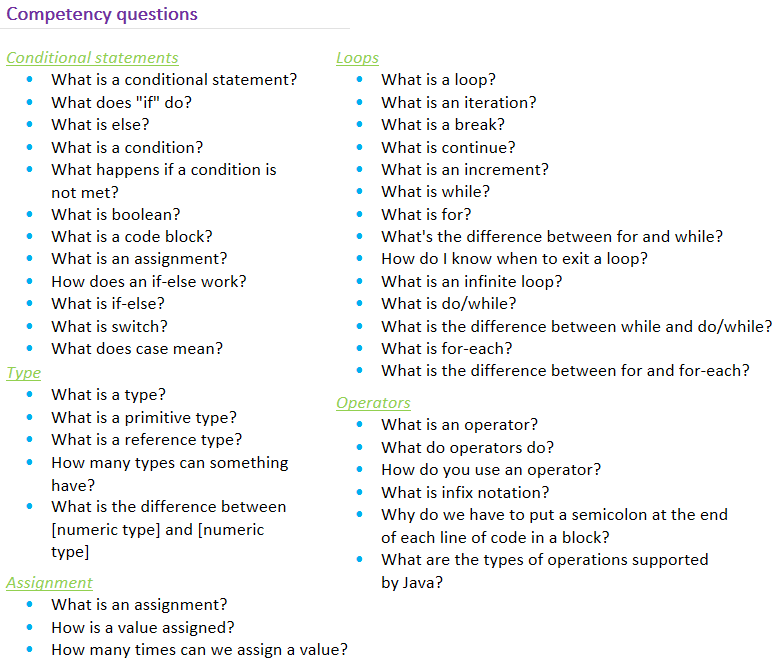
\includegraphics[scale=0.7, center]{competency.png}
\caption{List of Competency Questions (per category)}
\end{figure}
\newline
At the advice of Dr. Al-Sudani, I check whether the reasoner can answer a few targeted questions at a time, and when it manages to answer all the selected questions, I move on to another few. I select the questions based on category, which allows me to concentrate on one sub-topic at a time.

%step 3
\subsubsection{Initial Structuring}
This is the step where the lightweight ontology is created. This is a human-comprehensible representation of the knowledge model, and having such a structure in place allows for a clean formalisation of the software.
\newline
I started working on this model by taking a top-down approach, where I considered the general topic and went into further detail for each sub-topic. This lead to the creation of a mind map, which resembles a visual semantic network. The software used to create this map is provided by Mural\cite{mural}, and a copy is available in Appendix B.
\newline
While this is a very informative approach, it is by far not the best one to model the lightweight ontology. It does not cover the proper relation in between classes. Therefore, I only used it as an initial stepping stone in the process of building something a little more formal.
\newline
Following this visual, I created a UML diagram which allowed me to further formalise the class hierarchy and the relations between them. For this step, I used Enterprise Architect, a software tool that specialises in visual representations\cite{enterprisearchitect}.
\newline
\begin{figure}[h!]
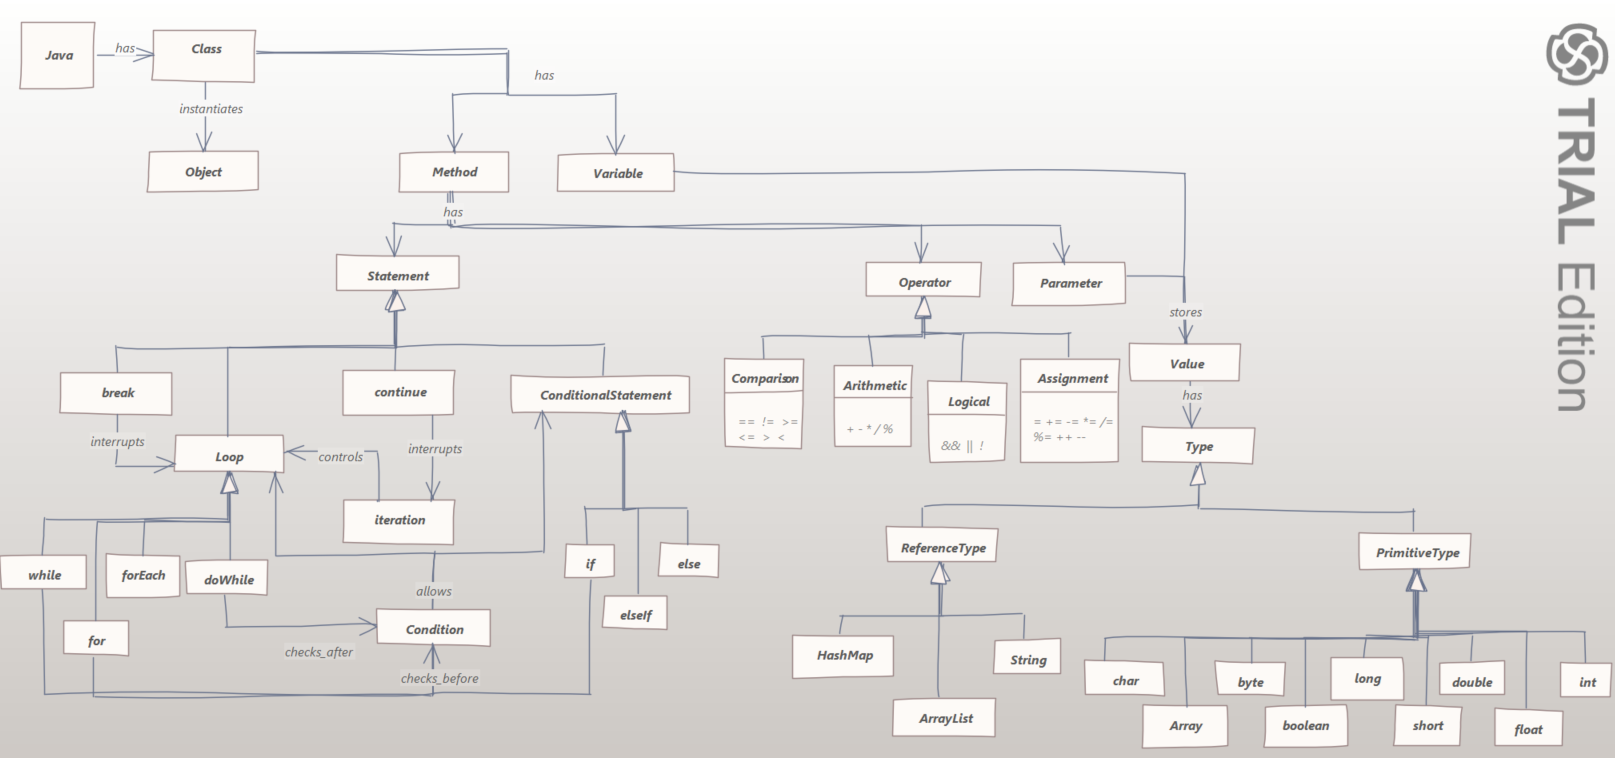
\includegraphics[scale = 0.55, center]{uml.png}
\caption{Formal Domain Structure: UML}
\end{figure}
\newline
As seen in the figure above, this visualisation is cleaner and it better defines the taxonomy. This model covers all the sub-aspects of Java statements.
\newline
In the following steps, I plan to further enhance this model by making it as accurate and simple as possible and by adding some more sub-topics of Java.

%step 4
\subsubsection{Formalization}
I started developing the formalised ontology using the Prot\'eg\'e 5.5.0 environment and OWL as the development language.
\newline
The current stage of the ontology consists of twelve main classes which have a combined total of 31 subclasses, all of which are properly disjoint and commented.
\newline
Alongside these, there are 22 properties (relationships), including inverses. Every property has been rightfully characterised (as irreflexive, asymmetric, functional, or inverse-functional, according to case). The fact that this ontology is so rigorous allows just enough room for the reasoner to make correct inferences. Currently, I am working towards modelling the available knowledge in such a manner that the competency questions can be accurately answered.
\newline
The latest task accomplished on the formal ontology was choosing a reasoner. The purpose of a reasoner is to ensure that all the classes from the ontology can be instantiated without problems and that there are no inconsistencies in the logic behind the development, as well as to create inferences on the ontology.
\newline
The original choice for the reasoner was Racer\cite{racerhome}, which was recommended to me by Dr. Al-Sudani. However, due to its deprecation in the more recent versions of Prot\'eg\'e, I have chosen HermiT 1.4.3.456, a top reasoner that became very popular in knowledge reasoning over the recent years\cite{hermithome}.
\newline
Since the tutoring system needs to be ``intelligent'', rather than giving it all the necessary information, I am allowing the reasoner to infer a few details of properties. Such an example would be having an inverse property and letting the reasoner infer the domain and the range. The only case in which HermiT cannot infer one of these sets is when they are created as disjunctions of classes.
\newline
On the topic of instances, I have decided, at least for now, not to add any. I was going to represent some explicit terms as instances, however there was an issue: an instance cannot be assigned a propety. In other words, if I were to take a term from the pool and make it an instance, I could not create a relation in between it and something else. For example, if the \texttt{for} statement was an instance rather than a class, I could not have added the fact that it is a kind of statement that checks a condition before executing an iteration (unlike \texttt{do/while}), or that it can be interrupted in different ways by using the \texttt{break} and \texttt{continue} statements.
\newline
As the ontology is still growing, I am using Dr. Chungoora's course, as well as ``A Practical Guide To Building OWL Ontologies''\cite{owlprotg}, to tackle any appearing problems and learn how to further develop the knowledge base. The current components of the ontology can be found at the end of this section.

%steps 5 and 6
\subsubsection{Deployment \& Evaluation}
These refer to testing and feedback, which is planned to start around the January examination period. In the lifecycle of ontology development, the purpose of these steps is to help refine the ontology until it answers the competency questions accurately and comprehensively.
\begin{figure}
    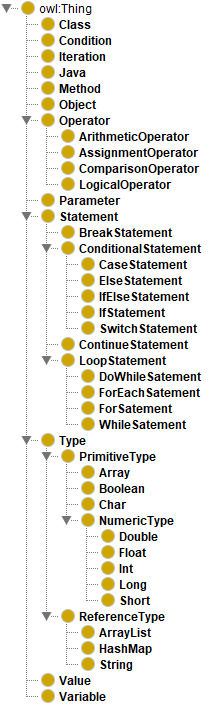
\includegraphics{classes.png}
    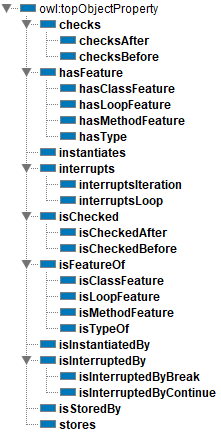
\includegraphics{properties.png}
    \caption{Current Classes and Properties of the Ontology}
\end{figure}
\newpage
\subsection{Building the Intelligent Tutoring System}
This requirement is met by a website that I am going to build until the following meeting. I want to implement a front end that has a selection of buttons representing competency questions to be answered by the reasoner.
\newline
I have not yet chosen the technology for the front end. Mainly, I would have liked to use React.JS, but Java is a smarter technology to use here as it would allow for a smoother link between the front and back end. Every other component of the design already uses Java.
\newline
The domain model is vital for the existance of the tutoring system, which means that it took higher priority in development. While I am enhancing the domain model however, I want to start working on the front end as well, and by the time of the next progress meeting in February, I want to have a solid beta version of the deliverables.

\section{Future Additions}
The first future step is to finalise the current version of the ontology so that most of the competency questions can be answered. During this time, I want to also create the front end and link it to the knowledge base. Once this system becomes functional, I want to enhance the knowledge model, and later go into more optional tasks and make the ITS visually pleasing.
\newline
Provided I can be granted this approval, I would like to work on some user input for the phases of deployment and evaluation. This would mean sending the software for testing to a group of individuals with different levels of experience. Each individual receives a package based on their level of familiarity with Java: the software and a level-based survey. A beginner would be asked questions such as how comfortable do they feel with Java and a quiz on some of the concepts, and someone more advanced can provide input on the system's scientific accuracy. Allowing individuals with different levels of experience to review the software would allow for well-rounded feedback.

\section{Conclusion}
The project is in the middle of development at the moment, and I have a very clear idea of what I want to work on next. While the ontology is not yet finalised, it manages to answer a number of competency questions, but in the future it will be able to answer even more. As there is no one correct way to develop this knowledge model, the current ontology will change over time, although most of the change will consist of additions rather than alterations.
\newline
The reviewed literature was very helpful in developing the formal ontology, and it also influenced the list of next steps in the design. As there are some different types new of components to be added, the literature list is going to contain some new references on Java web development and more general information on Intelligent Tutoring Systems.
\newpage

%References
\begin{thebibliography}{99}
\bibitem{aimaontology} Russell \& Norvig, 2016, Artificial Intelligence: A Modern Approach, Pearson; 3rd edition, p 308
\bibitem{wikikrr} \href{https://en.wikipedia.org/wiki/Knowledge_representation_and_reasoning}{Wikipedia.com}, Knowledge Representation and Reasoning
\bibitem{belgradepaper} Devedzic, 2001, Knowledge Modeling - State of the Art 
\bibitem{udemy} Chungoora, 2020, Practical Knowledge Modelling: Ontology Development 101, \href{https://www.udemy.com/course/practical-knowledge-modelling/}{udemy.com}
\bibitem{wikiontology} \href{https://en.wikipedia.org/wiki/Ontology_(information_science)}{Wikipedia.com}, Ontology (information science), Overview
\bibitem{semnet} \href{https://www.obitko.com/tutorials/ontologies-semantic-web/semantic-networks.html}{obitko.com}, Ontologies and the Semantic Web, Semantic Networks
\bibitem{golden} Golden, 2013, A Unified Formalism for Complex Systems Architecture, p 14
\bibitem{rulesvsonto} Czarnecki \& Sitek, 2013, Ontologies vs. Rules — Comparison of Methods of Knowledge Representation Based on the Example of IT Services Management, p 108
\bibitem{owlprotg} University of Manchester, A Practical Guide To Building OWL Ontologies Using Protege 4 and CO-ODE Tools, Edition 1.3
\bibitem{w3java} \href{https://www.w3schools.com/java/}{W3Schools.com}, Java
\bibitem{mural}\href{https://app.mural.co/}{Mural.co}
\bibitem{enterprisearchitect}\href{https://sparxsystems.com/}{Enterprise Architect}
\bibitem{racerhome}\href{https://www.ifis.uni-luebeck.de/~moeller/racer/}{The Racer Reasoner}, University of Lübeck
\bibitem{hermithome}\href{http://www.hermit-reasoner.com/}{The Hermit Reasoner}, University of Oxford
\end{thebibliography}
\newpage

\Large{\bf{Appendix}}
\appendix
\section{Initial Project Structuring}
\begin{figure}[h!]
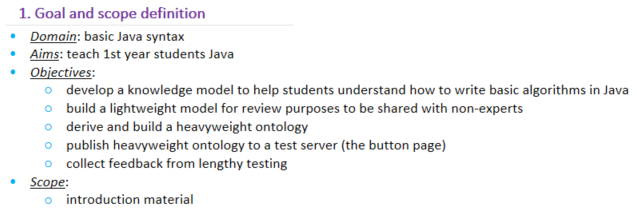
\includegraphics[scale = 0.9, center]{goal_scope.png}
\caption{Board of project initial structuring}
\end{figure}
\section{Initial Mind Map}
\begin{figure}[h!]
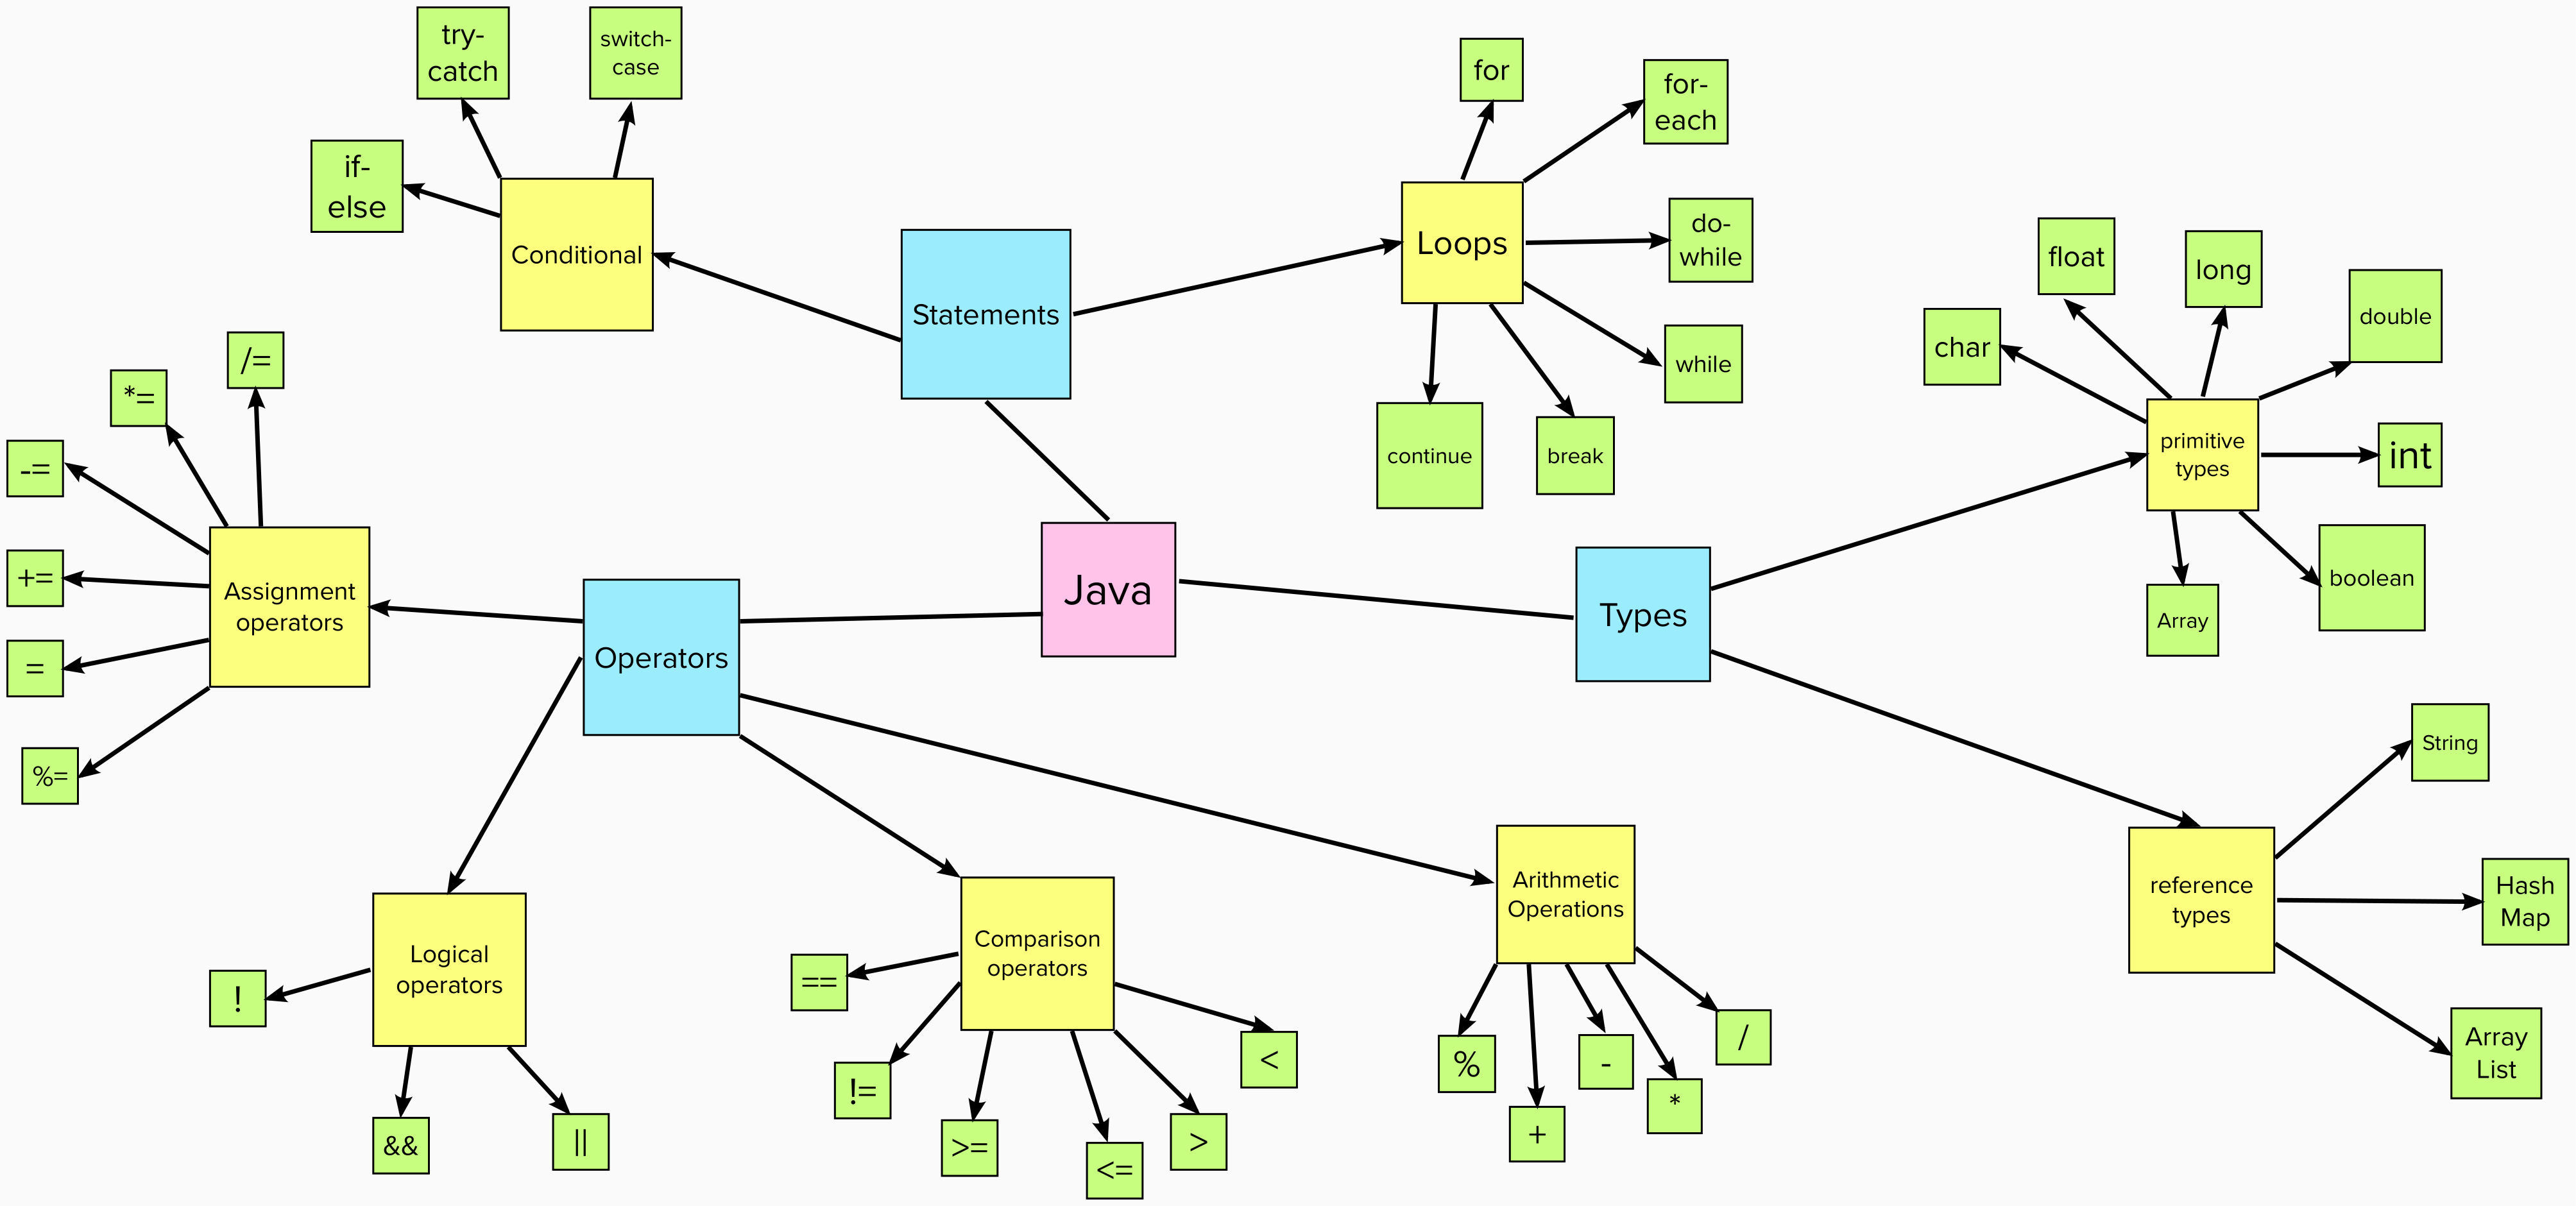
\includegraphics[scale = 0.095, center]{mural_latest.png}
\caption{Initial Domain Structure: Mind Map}
\end{figure}
\newpage
\section{Information Gathering Spreadsheet}
\begin{figure}[h!]
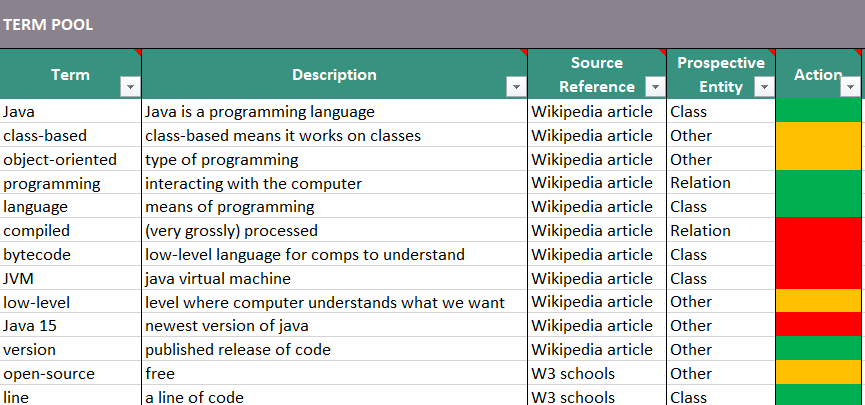
\includegraphics[scale = 0.7, center]{spreadsheet.png}
\caption{The Keyword Spreadsheet}
\end{figure}
\newpage
\end{document}